\chapter{Classifying SLSN using Machine Learning}
\label{Chapter5}
\lhead{Chapter 5. \emph{ML Classification}}

Throughtout this thesis, I worked with an underlying theme of performing SN classifications, focusing particularly on the selection of SLSN. In \cref{Chapter3}, I establised a definition of SLSNe in terms of the parameter space of the spin-down of a Magnetar model, later used to photometrically classify one SLSNe in the SNLS archival data. In this chapter, I start by describing these techniques as applied to the DES data set during the real-time search for SN in seasons two and three. This included both the manual scanning of SNe and combining it with the Magnetar model fitting. While successful in identifying several, later confirmed, candidate SLSNe, a number of misclassifications highlighted a need for a more robust approach.

In recent years the whole field of astronomy entered a new data analysis renaissance, utilising the Big Data tools and Machine Learning techniques to extract more from archival data and prepare for the arrival of new surveys such as Gaia, LSST, SKA that are expected to produce stagering amounts of data. These are not only difficult to handle for astronomers used to working on much smaller data samples but will infact require absolute state-of-the-art facilies and tools to handle and analyse the data streams. Following this revolution, I endevored to apply some of the latest techniques in ML to the problem of SN classification.

To date, there has been a number of SN studies aiming at classifying SN with the help of ML. Here, I am focusing only on the studies classifying the light curves of SNe and not point source classification pipelines such the once used in DES \citep{Goldstein2015} and Suburu \citep{Morii2016}. Amongst a number of similar works \citep{Karpenka2012,Moller2016,Charnock2016} the most thorough and indepth study of ML classification of SNe is presented in \citet{Lochner2016}. In their work, a number of models are used to extract a range of light curve features. They also provide a comparison of a number of Supervised ML algorithms and discuss their merits in terms of SN classification. While thorough in their analysis, their approach is not ready for deployment in a real survey. The training sampled used in their analysis is the SPCC dataset containing a sanitised sample of SNe only. In a survey such as DES we would first have to separate SNe from other types of transients which, when considering ML techniques, can be performed at the same stage as the classification of SNe.

The use of the SPCC dataset, containg only 2000 SNe weighted to match their observed rates, by \citet{Lochner2016} along with all previous ML classification studies of SNe is one of their greatest drawbacks. In this thesis, I aim to provide the first SN classification study utilising a large (tens of thousands objects of each class), artificially generated sample of objects. With the size of the training sample I tackle the common issue with overfitting for the less common subclasses of SNe. Furthermore, by placing the SNe uniformally throughtout the DES observing season and at a wide range of redshifts, I introduce real survey inperfections including objects whoch suffer from season edge effects and low S/N.

One of the greatest differences between all previous studies and this thesis is the family of ML algorithms used. \citet{Lochner2016} used the SALT2 model, in the process commonly refered to in ML as Feature Extraction or Feature Engineering, to extract a set of parameters that describe the light curve. These are then fed into the machine learning algorithm to produce their classifications. In this thesis, I use Convolutional Neural Networks (CNN), an overwelmingly powerful technique which dominates in the world of commercial ML solutions. CNNs, described in detail in \sref{sec:CNN}, use the data directly as they building their feature sets as part of the learning process. The use of a such a complex ML tool is only possible thanks to the size of the training sample and the data augmentation described in \sref{sec:DataAugmentation}.

In this chapter, I describe the process of creating an artificial training sample of SNe for a majority of subclasses, based on the tools developed in \cref{Chapter4}, as well as AGNs and noise spikes which form the majority of transients detected by DES. I then describe the steps taken to apply the survey noise model to the otherwise smooth simulated data before interpolating and ugmenting it with the help of GPR, described in \sref{sec:GP}. Finally, I discuss the use of the CNN framework to provide a photometric classification for all transients detected by DES in the first four years of its operations.

\section{Search for SLSN in DES using a Non-ML}
Before using machine learning to find SLSN I have used the magnetar model in the same way as in \cref{Chapter2}. This did produce some results and resulted in the classification of a few SLSNe in the data, however, we then started finding objects which really did not fit the model at all and sometimes even had a Chi2 of 3000, as in the case of DES15S2nr. Because of this, we knew that we need to try a different approach.

\subsection{Manual scanning of Transients}
The machine learning approach to classifying SNe, described in this chapter, is not the only method I have used to identify SLSNe in DES. Throughout the live operations of the survey, I have perform magnetar model fitting to the live transients using a techique similar to that described in \cref{Chapter3}. This allowed me to successfully identify several objects which have later been targetted, and subsequently confirmed as SLSN, using our spectroscopic follow-up facilies. However, it quickly became apparent that the there is a number of drawbacks to this technique which eventually led me to pursue the ML apprach as a more robust solution to this problem.

\subsection{Magnetar Model Fitting}
A major difference between the approach used to identify SLSN in DES and SNLS using the magnetar model fitting is the stage at which the data enters my pipeline. In \cref{Chapter3} I have applied the techniques retrsopectively to the archival data. This, other than in season edge cases, gave me a sample of near complete light curves which could be models with a much higher confidence rate. In DES, I attempted to model the light curves during their early rise phases. This was a constraint dictated not only by our wish to classify the objects at the earlierst possible phase (as the early spectra of SLSNe are still not sufficiently common) but also due to the computational resources required to fit all the light curves in real time. Despite a number of optimisations applied to our fitting routine (\sref{sec:SLAP}), I was only able to fit data detected within last three to four obsering epochs. As it is impossible to constrain such a complex model with less than three epoch of multi-band data, I have delayed the analysis of each objects until at least three observations in a minumum of three photometric bands are observed since the time of first detection. If the object was still active (i.e detected in the last of the tree epochs) I have attempted to fit the magnetar model to this object and compare it to the definition of SLSNe in the context of the parameter space of the magnetar model. I have then repeated this step up to four when new data was available for the object. If at that stage the object did not fit the definition it was discarded.

\subsubsection{Problems}
There is a number of problems involved with this approach to selecting SLSNe. All of which result in a number of objects that have been classified as SLSNe thanks to visual selection but have never been identifies as suitable candidates and conversely, objects which have been selected for spectroscopic follow-up and their classification did not match the expected type.

\paragraph{`Bumpy' SLSNe}
One of the drawbacks of the rules put in place in order to optimise the fitting process and reduce the number of false detections being passed through the fitting pipiline is the rejection of some objects, most prodominantly DES15C3hav, which show a slowly evolving pre-peak bump close to the detection limit of the survey (Angus et al; in prep). In the case of DES15C3hav, the early activity has only been detected in two consecutive epochs before the S/N of the object dropped considerably a number of weeks before its rebrightening at the onset of the main SLSN event. While no such cases have been recorded, it is also likely that a pre-peak bump similar to that found in DES14X3taz would have been excluded as the iniatial seven epochs do not form a good fit to the magnetar model and do not fit the definition of SLSNe.

\paragraph{Faint SLSNe}
One of the most interesting discoveries DES made about the population of SLSNe is the abundance of objects which spectroscopically math SLSNe but can often be found at absolute liminosities as low as M$\sim$-19. From \citet{Inserra2018a} and \citet{Nicholl2014, Nicholl2017} we know that the evolution of SLSN, both in terms of the rise and decline time, is strongly linked to the luminosity resulting in different morphology of the fainter events. No such objects were present in the sample used in \cref{Chapter3}, resulting in the magnetar model definition being strongly biasad against such objects. A number of fainter SLSN, including DES14XXslp ..., were overlooked

\paragraph{Lack of late time data}
 Perhapse the most important one is my assertion that it is possible to model a SLSNe using its rise time data only. It has been shown in \citet{Inserra2013} and \citet{Inserra2018a} that SLSNe are most strongly characterised by their late time light curve. This became very apparent when DES15E2mlf was discovered as the most distant, spectroscopically confirmed SLSN at the point of its classification \citep{Pan2017}. Both visual inspections, the search described in this section as well as the standard DES SN template fitting have strongly suggested that the object is a SN\,Ia at z$\sim$0.3. The unusually fast evolution of a SLSN is counter-intui

\section{Training sample} \label{sec:TrainingSample}
In any ML project, the training sample used to build the classification model is its most import element. Regardless of the algorithm used without the correct samples the model will not be able to accurately label new data and often may fall victim to overfitting. An ideal training set would be large compared to the number of distint classes, containing unambiguesly labelled objects and be indistinguishable from the unlabelled test sample that we wish to classify. In reality, this is difficult to achive and often involves manual scanning and classification of the training sample by the user (e.g the manual scanning of point source detection in DES \citep[][and similar studies]{Goldstein2015}).

In the case of SN light curves building the training sample is very difficult. The data comes from a very wide range of sources as the observations are taken using different telescopes, instruments and filters. The raw numbers of classified SNe are also insufficient with only several thousand objects classified to day [CITE?]. While commonly used, the SPCC dataset does not satisfy the requirement for a CNN training sample as the sample is too small.

In this thesis I, therefore, produce an artificial sample of objects that fit all of our requirements from first principles. For each class of object I determine the parameter space for their respective models that can be used to create a large quantity of perfect light curves in the DES photometric bands with an arbitraty cadence. I then apply the DES cadence and noise model to them, creating simulated survey events that closely resembles the real objects.

\subsection{DES Noise Model} \label{sec:NoiseModel}
The noise model applied to the data in this chapter is based heavily on the routines implemented in the SNANA package \citep{Kessler2009}. SNANA is a very powerful package designed as a tool for a realistic light curve simulations. It was used to simulate the SPCC data set \citep{Kessler2010} as well as generating a sample of SN\,Ia used to determine observational biases in the DES SN cosmology study [WHO DO I CITE; in prep.]. However, due to the design of the package, it is very difficult to implement further models into the code.

In DES, SNANA forms the backbone of the SN analysis and is used to extract the image quality logs from the science and reference frames; including the zero points, PSF and sky backgrounds amongst others. Internally these logs are refered to as the \textsc{SIMLIB} files. I follow the same procedure as implemented in SNANA to determine the uncertainty associated with an observation, given its mjd, observing field, filter and the CCD number. The final flux is then drawn randomly from a Normal distribution centered at the simulated flux, with a variance equal to the estimated uncertainty. To demonstrate the effectiveness of this approach, \fref{fig:IaNoiseComp} shows the comparison between the \textit{r}-band light curve of an example SN\,Ia observed by DES and a simulated light curve denerated based on a SALT2 model (performed using the SNCosmo package \citep{Barbary2014}) fit to the original object. The S/N ratio of the observed and simulated light curves fall close to unity, demonstrating their agreement.

\begin{figure}
  % \includegraphics[width=\textwidth]{/path/to/figure}
  \caption{\textit{Top}: \textit{r}-band light curve of an example SN\,Ia observed by DES and a simulated object created to replicate the original data point. \textit{Bottom}: the ratio of the S/N for the observed and simulated data light curves shown to be in agreement.}
  \label{fig:IaNoiseComp}
\end{figure}

\subsection{SN\,Ia}
Amonst the various SN classes simulated in as part of this thesis, SN\,Ia are unquestionably the most well-studied and understood class of objects. Thanks to over two decades of use as cosmological probes, there exists a number of packages able to model and simulate these objects with a high accuracy. Furthermore, the paramater spaces of SN\,Ia as well as peculiar outliries to the class (SN\,Ia-91bg and SN\,Ia-91T) are well understood, gives us a great starting point for our simulations.

While it would be possible to perform our own simulations, starting with any implementation of the SALT2 model (e.g SNANA, SNCosmo or otherwise), and pass these through the DES noise model (\sref{sec:NoiseModel}), I would essentially be replicating the sample of fake SN\,Ia injected into the science images during the live data reduction stages. In DES, these objects are used to estimate the image quality and generate the \textsc{SIMLIB} files making them equivalent to light curve that would be generated through SNANA.

The light curves of SN\,Ia that are injected into the images are generated using the extended SALT2 model as used in \citet{Betoule2014}. The upper redshift range was set as z=1.4 ensuring that the sample is not limited by the simualted redshift. We expect that DES is able to detect SN\,Ia up to redshift z$\sim$1.3. The fake SNe are injected such as to match the rate evolution measured by \citet{Perrett2012}. 50,000 objects have passed the detection criteria and therefore form part of our training sample of SN\,Ia. \fref{fig:IaDist} shows the redshift distribution for the sample.

\begin{figure}
  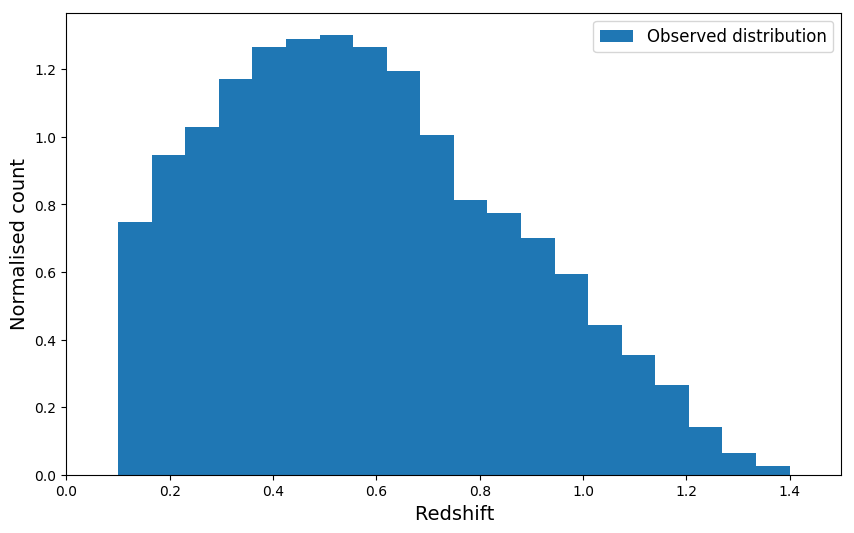
\includegraphics[width=\textwidth]{Figures/Chapter5/SNIa_z_dist.png}
  \caption{The redshift distribution of SN\,Ia that form part of our training sample. }
  \label{fig:IaDist}
\end{figure}

\subsection{CCSN}
The rate of CCSNe in the local universe is intrinsingly higher than the rate of SN\,Ia [CITE THE BOOK] in the local universe, with an approximate flaction of 70\% CCSNe to 30\% SN\,Ia. However, as CCSN are a fainter with an average brightness only a tenth of the SN\,Ia luminocity. As a result, survey such as DES we can only detect them up to the z$\sim$0.6 as opposed to z$\sim$1.3 for SN\,Ia, giving a much lower observed rate. In our study it was necessary for our sample not to replicate this observed rate as the training of a CNN required that all classes used in the classification are relatively equally represented.

While there is a great diversity amongst CCSNe in terms of both their morphology and peak luminocity, our simulation package, \textsc{CoCo} (\sref{sec:CoCo}), was designed to simulate their whole population. As the overarching aim of this thesis is the classification of SLSNe, as opposed to providing an accurate photometric classification for all transients detected by DES, an accurate treatment of the CCSNe could be considered excesive. The Nickel decay, powering mechanisms behind SN\,Ia and SN\,Ib/c, results in light curves which are often difficult to separate, giving rise to the original inspiration behind developing \textsc{CoCo}. A possible drawback of this could be overfitting of SN\,Ia and CCSNe if these two classes were found to be too alike. Contrarily, I would not wish to indruduce such bias into our training sample as the low redshift behaviour of the SNe may not necessarily be reflected for objects observed at higher redshifts when all observational factors are considered. The behaviour of the objects may also differ between SN\,Ib/c and SN\,II, hence in this chapter I build separate samples for these two classes of SNe both matching the SN\,Ia sample in size. In \sref{sec:CNN} I then consider performing SN classification by mixing these objects at various abundancies.

\subsubsection{SN\,Ib/c}
In \cref{Chapter4}, I presented a method for creating templates as well as simulating SN\,Ib/c. I have used \textsc{CoCo}, the package developed for this purpose to simualate over 100,000 objects based on the spectroscopic templates shown in \tref{tab:IbcTemplates}. Due to the low number statistics of the sample, the spectral subtypes of the templates do not match their measured relative abundance. Following Firth et al. (in prep), I use the \citet{Li2011} measurement of the local rates of CCSNe to correct their abundancies. A question was raised as to whether the subclasses should be represented equally thoughout the sample or match their observed rates. I made the decision to follow their observed abundancies as we are not interested in assigning subclasses to these SNe. Furthermore, some subclasses are very ill-represented in our sample and would therefore be replicated more than other objects likely leading to model overfitting.

\begin{table}
  \caption{}
  \label{tab:IbcTemplates}
  \centering
  \begin{tabular}{l|r|r}
    SN Name  & redshift & count \\
    \hline
    SN1993J  & 0.79 & 1263 \\
    SN1994I  & 0.70 &  313 \\
    SN1996cb & 0.78 &  945 \\
    SN1998bw & 0.80 & 6151 \\
    SN2002ap & 0.80 & 1271 \\
    SN2005bf & 0.80 & 3660 \\
    SN2005hg & 0.80 &  887 \\
    SN2006aj & 0.80 & 5002 \\
    SN2007Y  & 0.57 &  146 \\
    SN2007gr & 0.67 &  345 \\
    SN2007uy & 0.64 &  263 \\
    SN2008D  & 0.28 &   38 \\
    SN2008ax & 0.43 &  208 \\
    SN2008bo & 0.46 &  108 \\
    SN2009iz & 0.80 &  623 \\
    SN2009jf & 0.80 & 1844 \\
    SN2010al & 0.80 & 5008 \\
    SN2011bm & 0.80 & 7554 \\
    SN2011dh & 0.73 &  964 \\
    SN2011ei & 0.39 &  105 \\
    SN2012ap & 0.54 &  191 \\
    \hline
  \end{tabular}
\end{table}

I generate the light curves in the redshift range of 0$<$z$<$0.8, drown using a volume weighted, non-uniform random distribution corresponding to the star formation rate of the universe \citep{Hopkins2006}. To introduce a level of diversity into the sample, I apply host galaxy reddening to the templates (Milky Way extinction is not necessary as DES observed is very low extinction fields). I use the \citet{Cardelli1989} law with R$_\mathrm{v}$=3.7 and the A(B-V) values drawn randomly from the modulus of a Normal distribution centered at zero with a variance, $\mu$=0.2. Furthermore, I have used a similar (but unmodulated) distribution to apply an offset to the peak magnitude of the SNe. This is, again, aimed at introducing a scatter into the training sample as the low number of available templates, despite being placed at different redshifts and explosion dates, would produce a sample of repeating objects that yet again could lead to overfitting.

From the simulations we measure the detectibility of each template as the function of redshift (see \tref{IbcTemplates}) as well as the detection frequency of the whole population as a function of redshift shown in \fref{fig:IbcDist}. As expected SN\,Ib/c are detectable only up to z$\sim$0.8 which is significantly lower than that of SN\,Ia (\fref{IaDist}).

\begin{figure}
  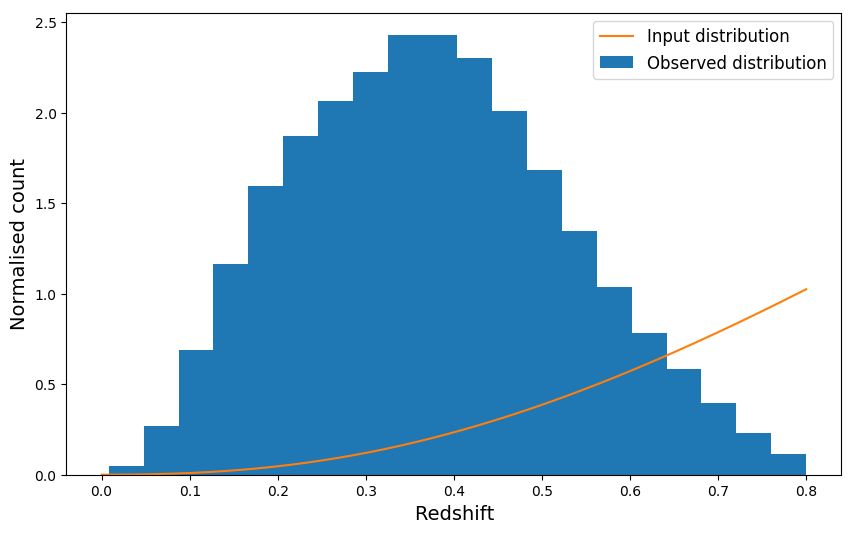
\includegraphics[width=\textwidth]{Figures/Chapter5/SNIbc_z_dist.png}
  \caption{}
  \label{fig:IbcDist}
\end{figure}

\subsubsection{Hydrogen-Rich SN}
The method used for building the training sample of SN\,II followed that of SN\,Ib/c very closely. I used the template sample, generated using the \textsc{CoCo} package, as present in \tref{tab:SNIITemplates}. The only significant difference in the process of generating the sample was the simulated redshift range which was increased to z$\sim$0.9 as we have found during our testing that using z<0.8 would result in a number of objects being detected at the upper redshift limit.

\begin{table}
  \caption{}
  \label{tab:SNIITemplates}
  \centering
  \begin{tabular}{l|r|r}
    SN Name  & redshift & count \\
    \hline
    SN1999el & 0.40 &  4052 \\
    SN2000cb & 0.36 &  4127 \\
    SN2000eo & 0.78 & 20895 \\
    SN2002gd & 0.26 &  1924 \\
    SN2006V  & 0.45 &  7178 \\
    SN2007pk & 0.75 & 18822 \\
    SN2009E  & 0.30 &  3538 \\
    SN2010al & 0.90 & 30882 \\
    SN2011hs & 0.26 &   792 \\
    SN2012ec & 0.36 &  5176 \\
    SN2013ej & 0.36 &  4114 \\
    \hline
  \end{tabular}
\end{table}

From \tref{tab:SNIITemplates} we see that there is a bimodality in the detectibility o the training sample whereas most of the objects are detectable only at low redshhift with three templates being detected at a significantly greater redshift. As a result these objects have a much higher frequency of detection in my simulations, scewing the detection distribution (\fref{fig:IIDist}). This, again, may cause serious overfitting issues. However, as I generate an overabundance of points, in \sref{sec:CNN} I investigate different combinations of the training samples including one where I select it uniformally based on the original template the simulation was based on.

\begin{figure}
  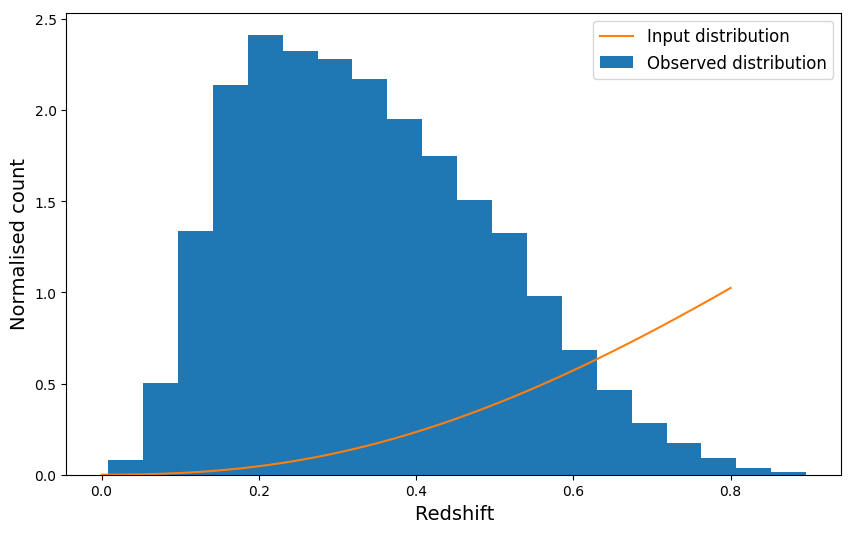
\includegraphics[width=\textwidth]{Figures/Chapter5/SNII_z_dist.png}
  \caption{}
  \label{fig:IIDist}
\end{figure}

\subsection{SLSN}
The simulations of SLSNe have been one of the most challenging parts of this thesis. The low number of known examples of the class, combined with the uncertainty surrounding their definition and the engine powering their staggering luminocity makes the modelling of these objects a challenging task. In the case of their simulations, for the purpose of a classification study such as the one presented in this thesis, we must not only replicate all previosly observed objects but also make a reasonable, but not overly constraining, prediction for what SLSN may appear as and represent as a class. Until very recently, this would have not been possible as our understanding of the models of SLSNe, and their parameters was not sufficient. However, several works including \cref{Chapter3,Chapter4} of this thesis as well as \citet{Inserra2013,Nicoll2013,Nicoll2017} and Angus et al. (in prep) showed that the spin-down of a Magnetar model is able to describe all SLSNe with an acceptable level of accuracy.

The greatest step towards simulating SLSNe was achived in \citet{Inserra2018a} where we have established their new definition that is versitile and robust enough to produce a sample that matches all observed objects but at the same time is limited in the span such that it does not overlap with other classes of SNe. This definition is based on Four Observables Parameter Space (4OPS), defined in narrow (800\AA and 1000\AA wide respectively) box filteres centered at 4000\AA and 5200\AA, by; the peak in the 4000\AA band light curves, colour between the band at peak and +30 days post maximum, and the drop in magnitude between the peak and +30 days in the 4000\AA band. \citet{Inserra2018a} finds that SLSNe form linear correlations in this paramater space, with a narrow scatter shown in \fref{fig:4OPS}. I use this property to determine the magnetar model parameters which correspond to the definition of SLSNe.

\begin{figure}
  % \includegraphics[width=\textwidth]{/path/to/figure}
  \caption{}
  \label{fig:4OPS}
\end{figure}

I simulate a large number of SLSNe using the magnetar model and compare them to the 4OPS definition. The magnetar model parameters are drawn randomly from a uniform top-hat distribution, bound at 10<$\tau_M$<150, 0.1<$B_{14}$<20.0, 0.01<$P_{ms}$<10.0. These limits were informed by the definition of SLSNe used in the rate calculation described in \cref{Chapter3}, but was expanded to ensure completeness but, at the same time, limit the number of computationally expensive simulations that needed to be performed. I have also introduces a modification to the 4OPS definition of SLSNe, similar to that in Angus et al. (in prep), where as the parameter spaces are expanded by one magnitude of scatter while retaining the original slope of their relationship. This was aimed at including fainter objects such as those found in the DES spectroscopically confirmed sample (\sref{sec:DES_SLSN}), that were not available at the time the relationship was constructed. The modified limits are presented in \tref{tab:4OPS} and can be seen in \fref{fig:4OPS} along with the regions where objects drawn from the magnetar model.

\begin{table}
  \caption{}
  \label{tab:4OPS}

\end{table}

\begin{figure}
  % \includegraphics{/path/to/figure}
  \caption{}
  \label{fig:4OPSMag}
\end{figure}

In \fref{fig:4OPSMag}, I show the distribution of magnetar model paramaters that result in objects that match the 4OPS definition of SLSNe. Perhapse the most interesting result is the luminocity function that results from drawing objects uniformly from the magnetar model parameter space. With no external inputs, the functions matches that observed by \citet{DeCia2017} in the PTF sample of SLSNe. I use the sets of magnetar model parameters that match the SLSN definition to generate the training sample of SLSNe for the use in \sref{sec:CNN}. In total $\sim$100,000 SLSN were generated at a range redshifts with 0<z<3, drawn from a volume weighted distribution following the start formation rate of the universe \citep{Beacon2004} similarly to CCSNe (\fref{fig:SLSNDist}).

\begin{figure}
  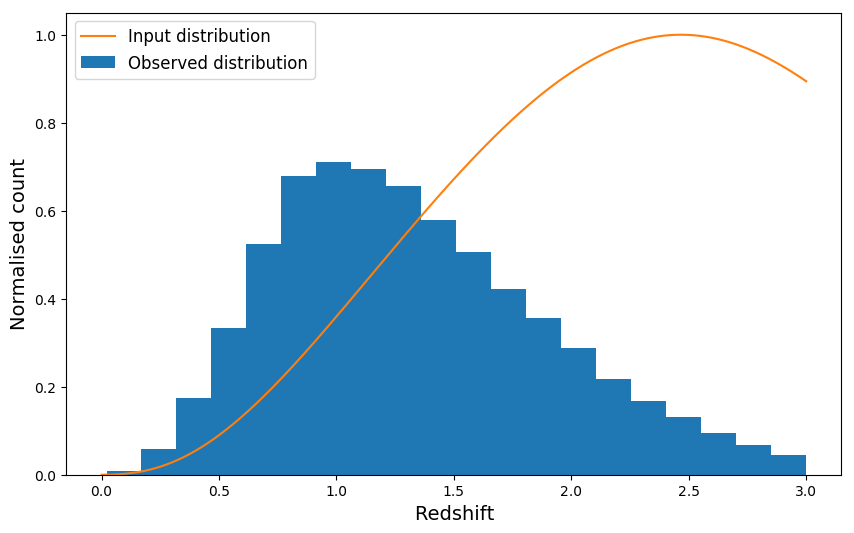
\includegraphics[width=\textwidth]{Figures/Chapter5/SLSN_z_dist.png}
  \caption{}
  \label{fig:SLSNDist}
\end{figure}

\subsection{AGN}
Active Galactic Nuclei (AGN) are the largest contaminant in the DES sample. This is only partially due to their physical morphology but in greater measure the design of the survey. AGNs are most commonly associated with long, quasi-periodic, variable light curves that are often easy to identify based on their historical variability. As no long-term observations, matching its depth, are available for the DES SN fields making each first AGN detection its discovery. Prior to the first season of DES, a set of science verifiction images were taken which were used as templates in the image supraction pipeline used to detect new transients. AGNs that have undergone rebrightening in the first season were detected as potential supernova candidates. If the templates remained unchanged for the duration fo the survey we would see a decrese in the contamination each season. Furthermore, we would be able to remove most of these transients restrospectivaly by selecting objects with detections in multiple seasons. The survey did, however, change the templates each year in the first three seasons of DES to use the best images taken in the previous season. In the final two seasons the data from year two was used as templates. Additionally, the data for the first season was later reanalysed using season two as a template. A caveat of DES that caused us particular issues is that negative `detections' are not considered as detections within the transient selection algorithms. As a result, each DES season contains a large number of objects which are selected as new transients despite showing stong visual signs of prior, albeit `negative', variability.

In the cases of SLSNe, this is particularly troubling as their slow evolution can be sometimes confused with an AGN with a quasi-period of approximately one year, if only a single DES seasons are considered. It is, therefore, imparitive that AGNs are correctly represented in the ML training sample used in \sref{sec:CNN}. For this purpose, I use the existing simulations of AGNs, in the DES observing bands, presented in \citet{Honig2016}. While these simulations were originally aimed at evaluating the possibility of using AGNs as cosmological probes applying a technique called Reverberation Mapping, they were perfectly suited for this project. The simulated light curves did not contain any observed noise, were densely sampled (one day cadance) and had a span exceeding four years. In total 100,000 simulated objects were available for this study including those placed at redshifts outside the detectible range for DES. I have therefore placed each object at random start dates and fields, before applying the survey noise using the method described in \sref{sec:NoiseModel}, resulting in $\sim$60,000 detected AGNs.

\subsection{Noise}
Visual inspection of the DES light curve data shows that a limited number of objects, originally recognised as a real transient according to the DES transient selection criteria (\cref{Chapter2}), do not appear to be physical in origin. There appear to be two main origins for these objects: bad image subtractions and spurious noise detections. Despite a soffisticalted, ML powered, transient selection pipeline \citep{Goldstein2015}, some objects (often elongated and with negative subractions; \fref{fig:BadSubtractions}) can pass the ML cuts, albeit with a low score. In some cases, likely dependant on the observing conditions, this may occur in several epoch separated by less than 30 days, giving the object a `real transient' flag.

Another channel that can result in the misclassifications of candidates is the detection of slow-moving, near earth object. Such objects are most commonly detected at the same position only in two or three consecutive bands. In subsequent epochs, they are, in normal circumstances, no longer detected at the same position resulting in the object being rejected. However, in some rare cases, bad subtractions or random noise spikes exceeding the 5 sigma detection limit, within 30 days cut can result in a `real transient' flag.

\begin{figure}
  % \includegraphics{/path/to/figure}
  \caption{}
  \label{fig:BadSubtractions}
\end{figure}

To model these objects, I use a very simple approach of inserting a number of sharp, $\delta$-function like spikes in the data that correlated between the filters and separated by less than 30 days to account for the misidentifications. The spikes are selected between 19$<$mag$<$22 in order to test the different behavious of the GP interpolations used in the next step of this analysis (\sref{sec:DataAugmentation}). The absolute value of the peak does not play an important role in the classification process as the data is normalised before entering the CNN. Similarly to other classes of transients, $\sim$100,000 objects have been simulated across all fields.

\subsection{Missing classes}
While in this thesis, I have created one of the most thorough training samples of SNe for the purpose of a ML classification study, it still cannot be said to be complete. There are a number of classes of known transient objects which we were unable to accounted for in this work. Some objects such as kilonovae, associated with gravitational waves as their optical counterparts, evolve too rapidly to be using the cedence of DES. Omitting these (undetectable) events does not bring any difference to the final result of our classification. However, one class of objects which could have an effect on our final classification are the newly discovered class of rapidly evolving SNe \cite{Drout2014,Kepler2018}. Recent work by \citet{Pursiainen2018} showed that these objects are relatively common within DES with 72 detections in the first four seasons of its operations. While there are now early, tentitive, signs \citep{Pursiainen2018} that these objects are powered by a SN shock interacing within a thick an extended wind \citep{Piro2015}, similar to the model used in modelling of the `bumps' found in SLSNe \sref{sec:MagExtensions}. It is this particular connections that would be interesting to explore, however, the modelling of these objects is still in its infancy. The model parameter spaces defining them, their SED models and other simialar aspects developed for SLSNe over the last several years have not yet been studied for the fast evolving SNe.

The omission of rapidly evolving SNe from our sample will result in these objects being mislabelled in our classifications. It would however be unlikely that any of the objects that we have not included in the training sample would get mislabelled as a SLSNe due to their significanly faster evolution. I test this assertion in \sref{CNN} using the ground-truth sample of objects identified by \citet{Pursiainen2018}.

\section{Data Augmentation} \label{sec:DataAugmentation}
Before the training sample of SNe created in \sref{sec:TrainingSample} can be used to build a CNN classification model, it has to first undergo a number of augmentation steps. The data passed through the CNN must be uniform in terms of the number of points as well  their separation, regardless of the field and season the data was taken from. To achieve this, I first select a length of observations, then I choose a new cadance that will overlap most closely with that observed by DES before applying the flux correction required to normalise the effect of using a changing subtraction template in different season. Finally I use GPR in order to interpolate and augment the data such as to meet the requirements of CNN.

\subsection{Choosing the observing block} \label{sec:ObsBlock}
I define the observing block, for the used in our classification study, as the span of time (measured in days) that is the longest period over which an DES season observes any of its field. Due to the observing conditions and sheduling the DES observing seasons vary between the seasons and fields, with a difference can between the longest and shortest observing window measuring 40 days. This is not only caused by the sheduling or the observability of the fields but also due to the observing conditions as in the early parts of the season a large number of observations is lost to the cloudy conditions. This results in either large gaps in the data for all or several filters.

Selecting the observing block is not as straight foward as to simply use the length of the shortest season. \fref{fig:ObsBlock1,fig:ObsBlock2,fig:ObsBlock3,fig:ObsBlock4} show the cedance of DES in seasons 1-4 in all fields and bands.

This is done in two stages, first I find the span that covers all the filters. From the first point where all the filters are observed to the last point where all the filters are observed. I then remove the points at the start of the season where there is a gap in the data longer than 10 days. This happens in a few filters where an observation has been missed due to the atmospheric conditions. If a similar gap to this exists later on in the light curve the GPR interpolation can handle it well but at the start of the season there is not enough information to anchor the fit.

From these measurements I determine the optimal observing block to be 149 days in duration. The span covered by the block in each season and filter is shown in \fref{fig:ObsBlock1,fig:ObsBlock2,fig:ObsBlock3,fig:ObsBlock4}. Due to the improved qualityof the lightcurves in the second part of each season, I place the observing block as late in time as possible.

\begin{figure}[h]
  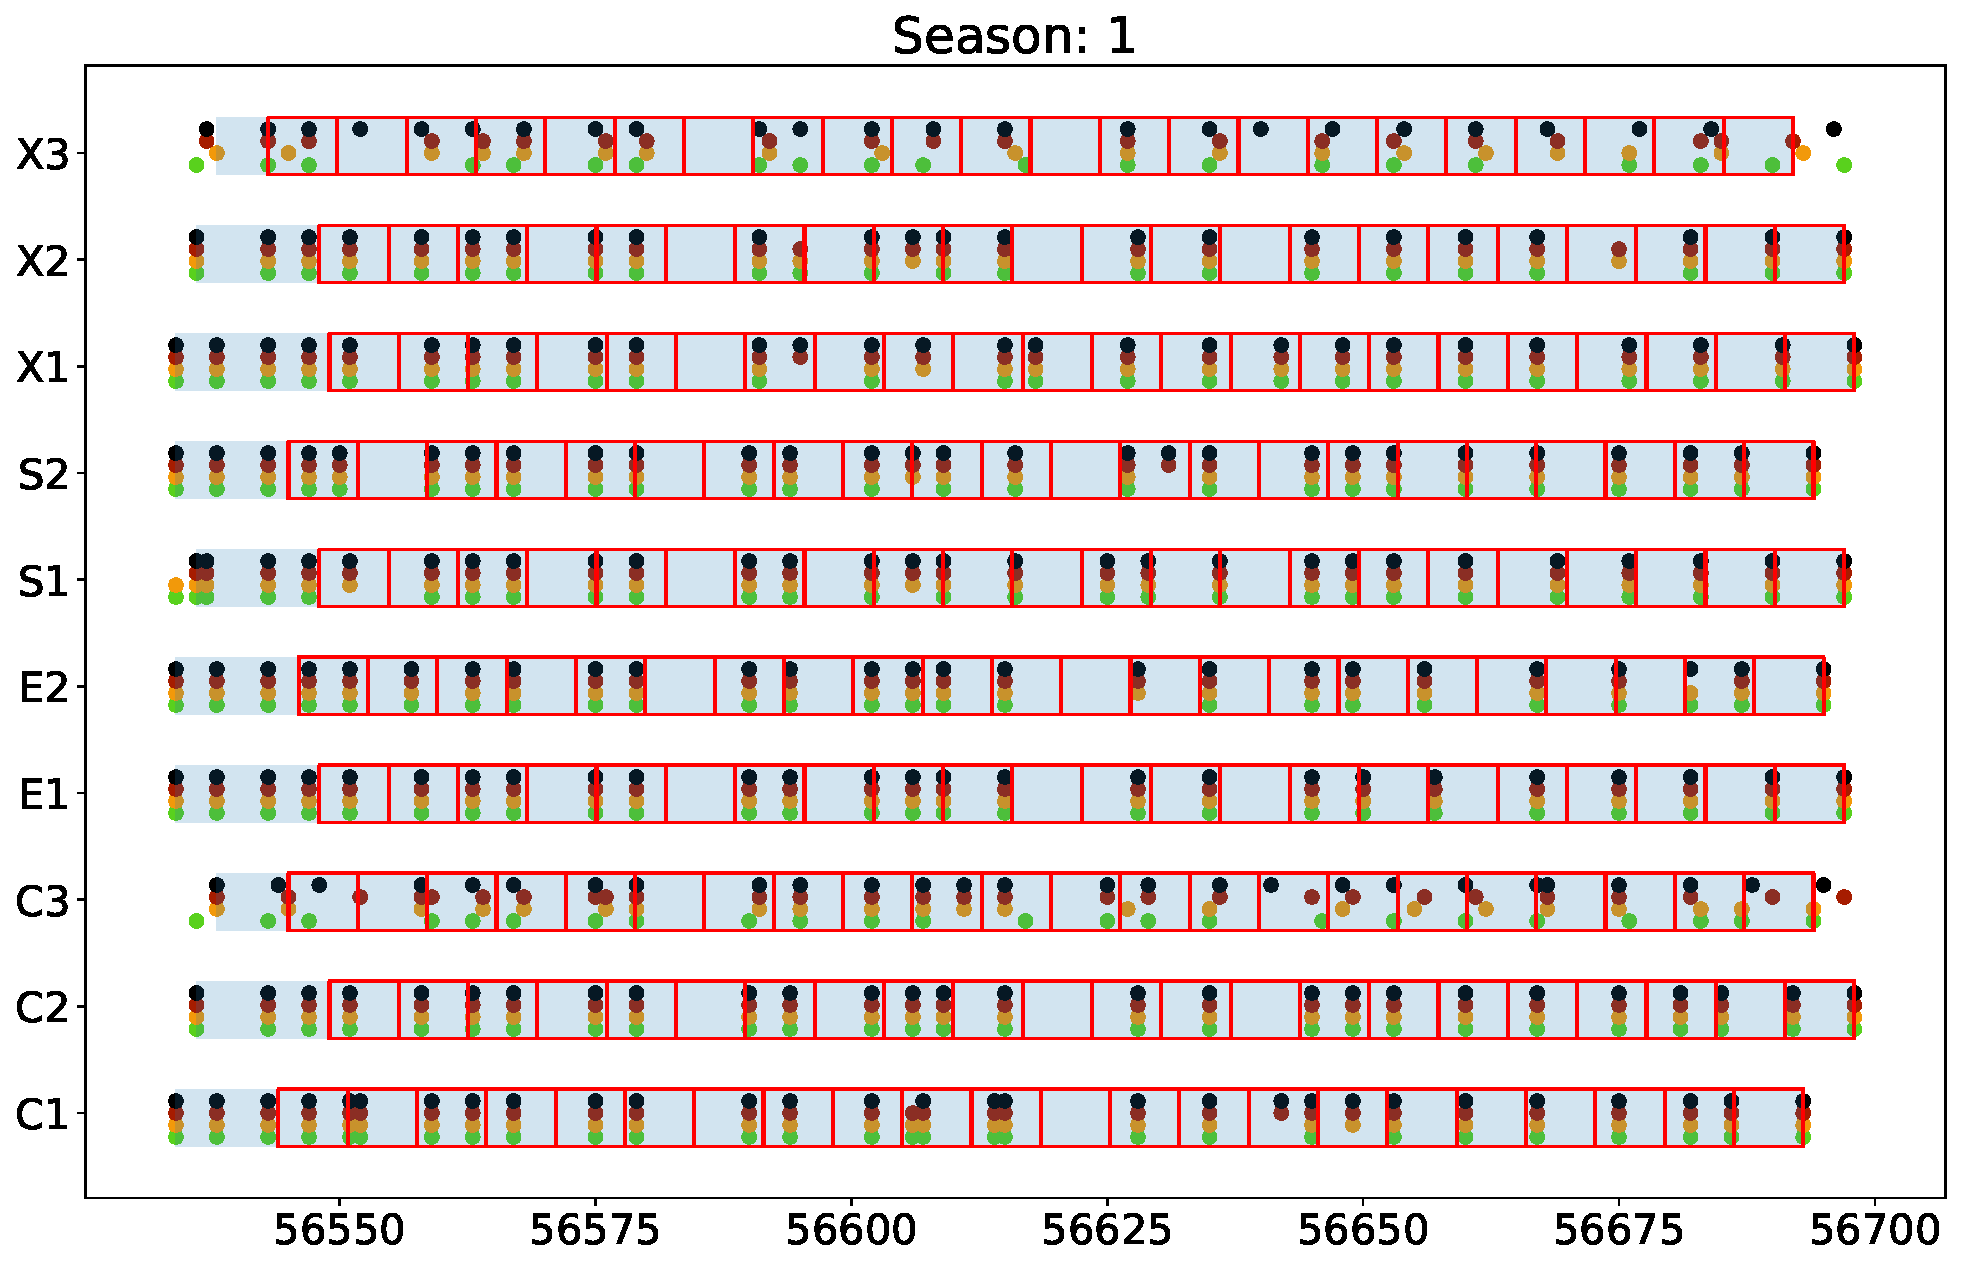
\includegraphics[width=\textwidth]{Figures/Chapter5/ObsBlock_Season1.pdf}
  \caption{}
  \label{fig:ObsBlock1}
\end{figure}

\begin{figure}[h]
  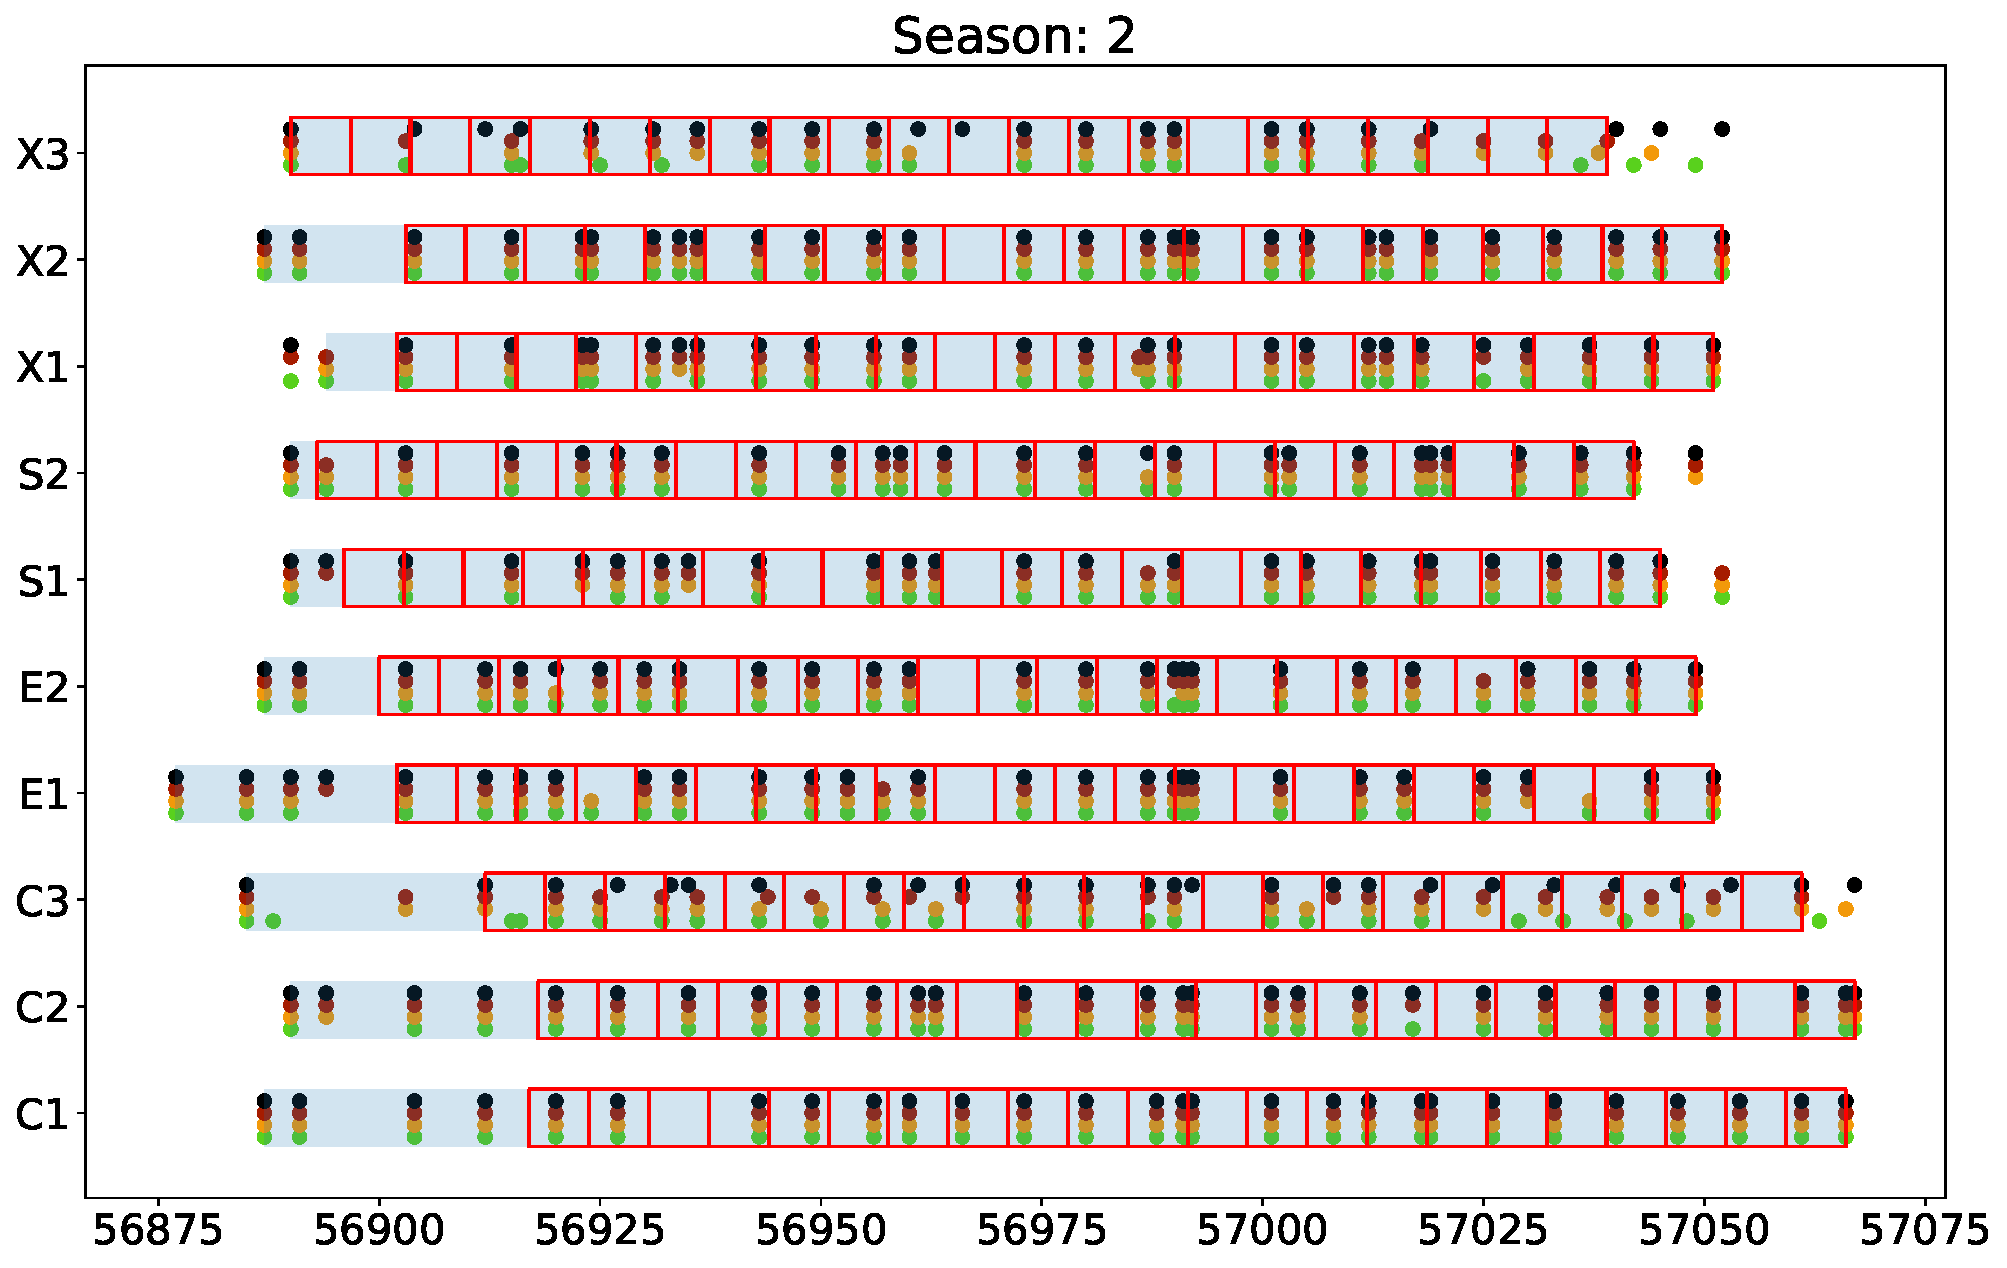
\includegraphics[width=\textwidth]{Figures/Chapter5/ObsBlock_Season2.pdf}
  \caption{}
  \label{fig:ObsBlock2}
\end{figure}

\begin{figure}[h]
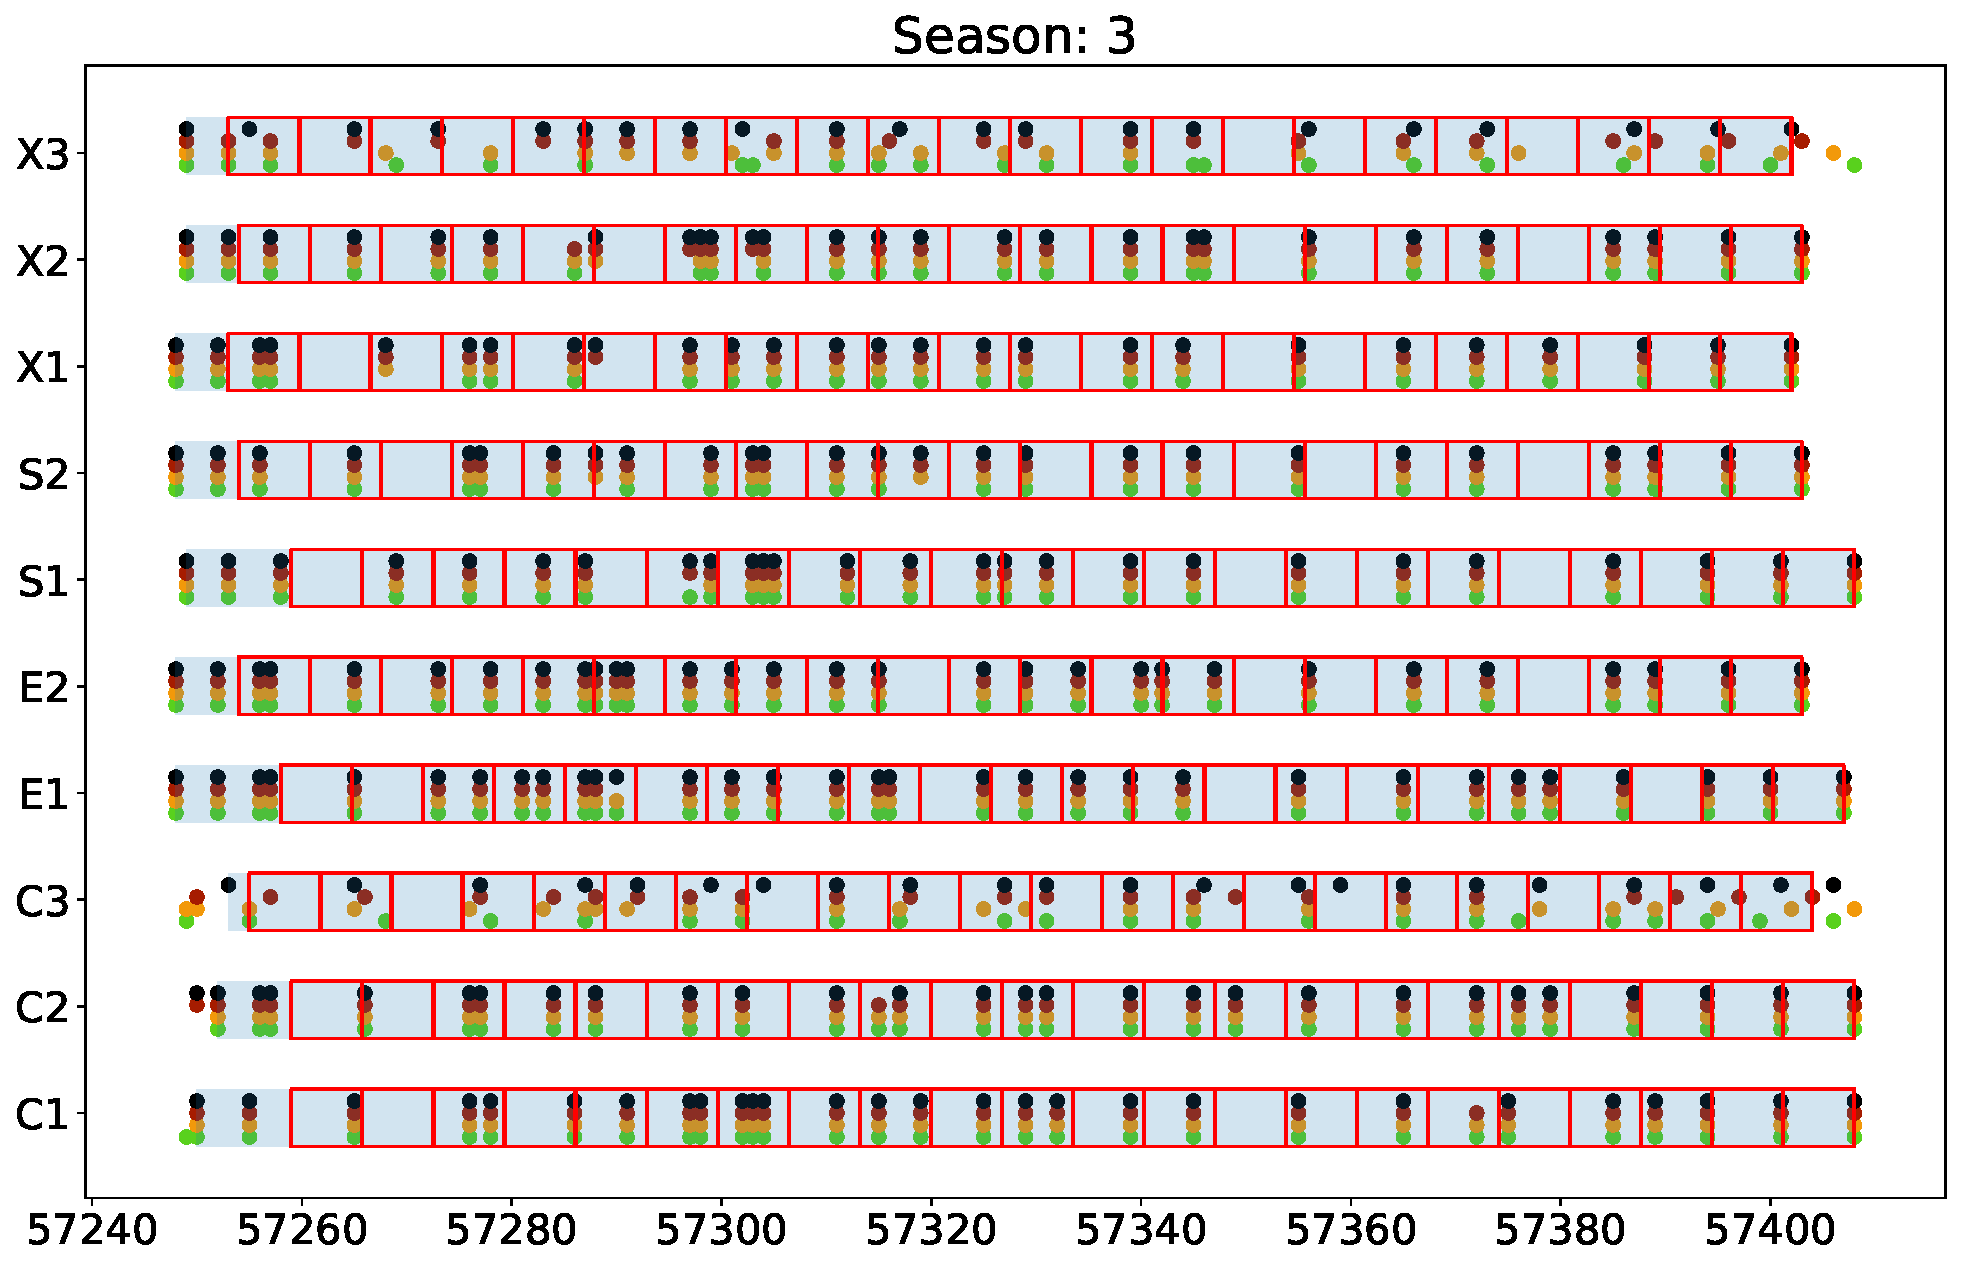
\includegraphics[width=\textwidth]{Figures/Chapter5/ObsBlock_Season3.pdf}
  \caption{}
  \label{fig:ObsBlock3}
\end{figure}

\begin{figure}[h]
  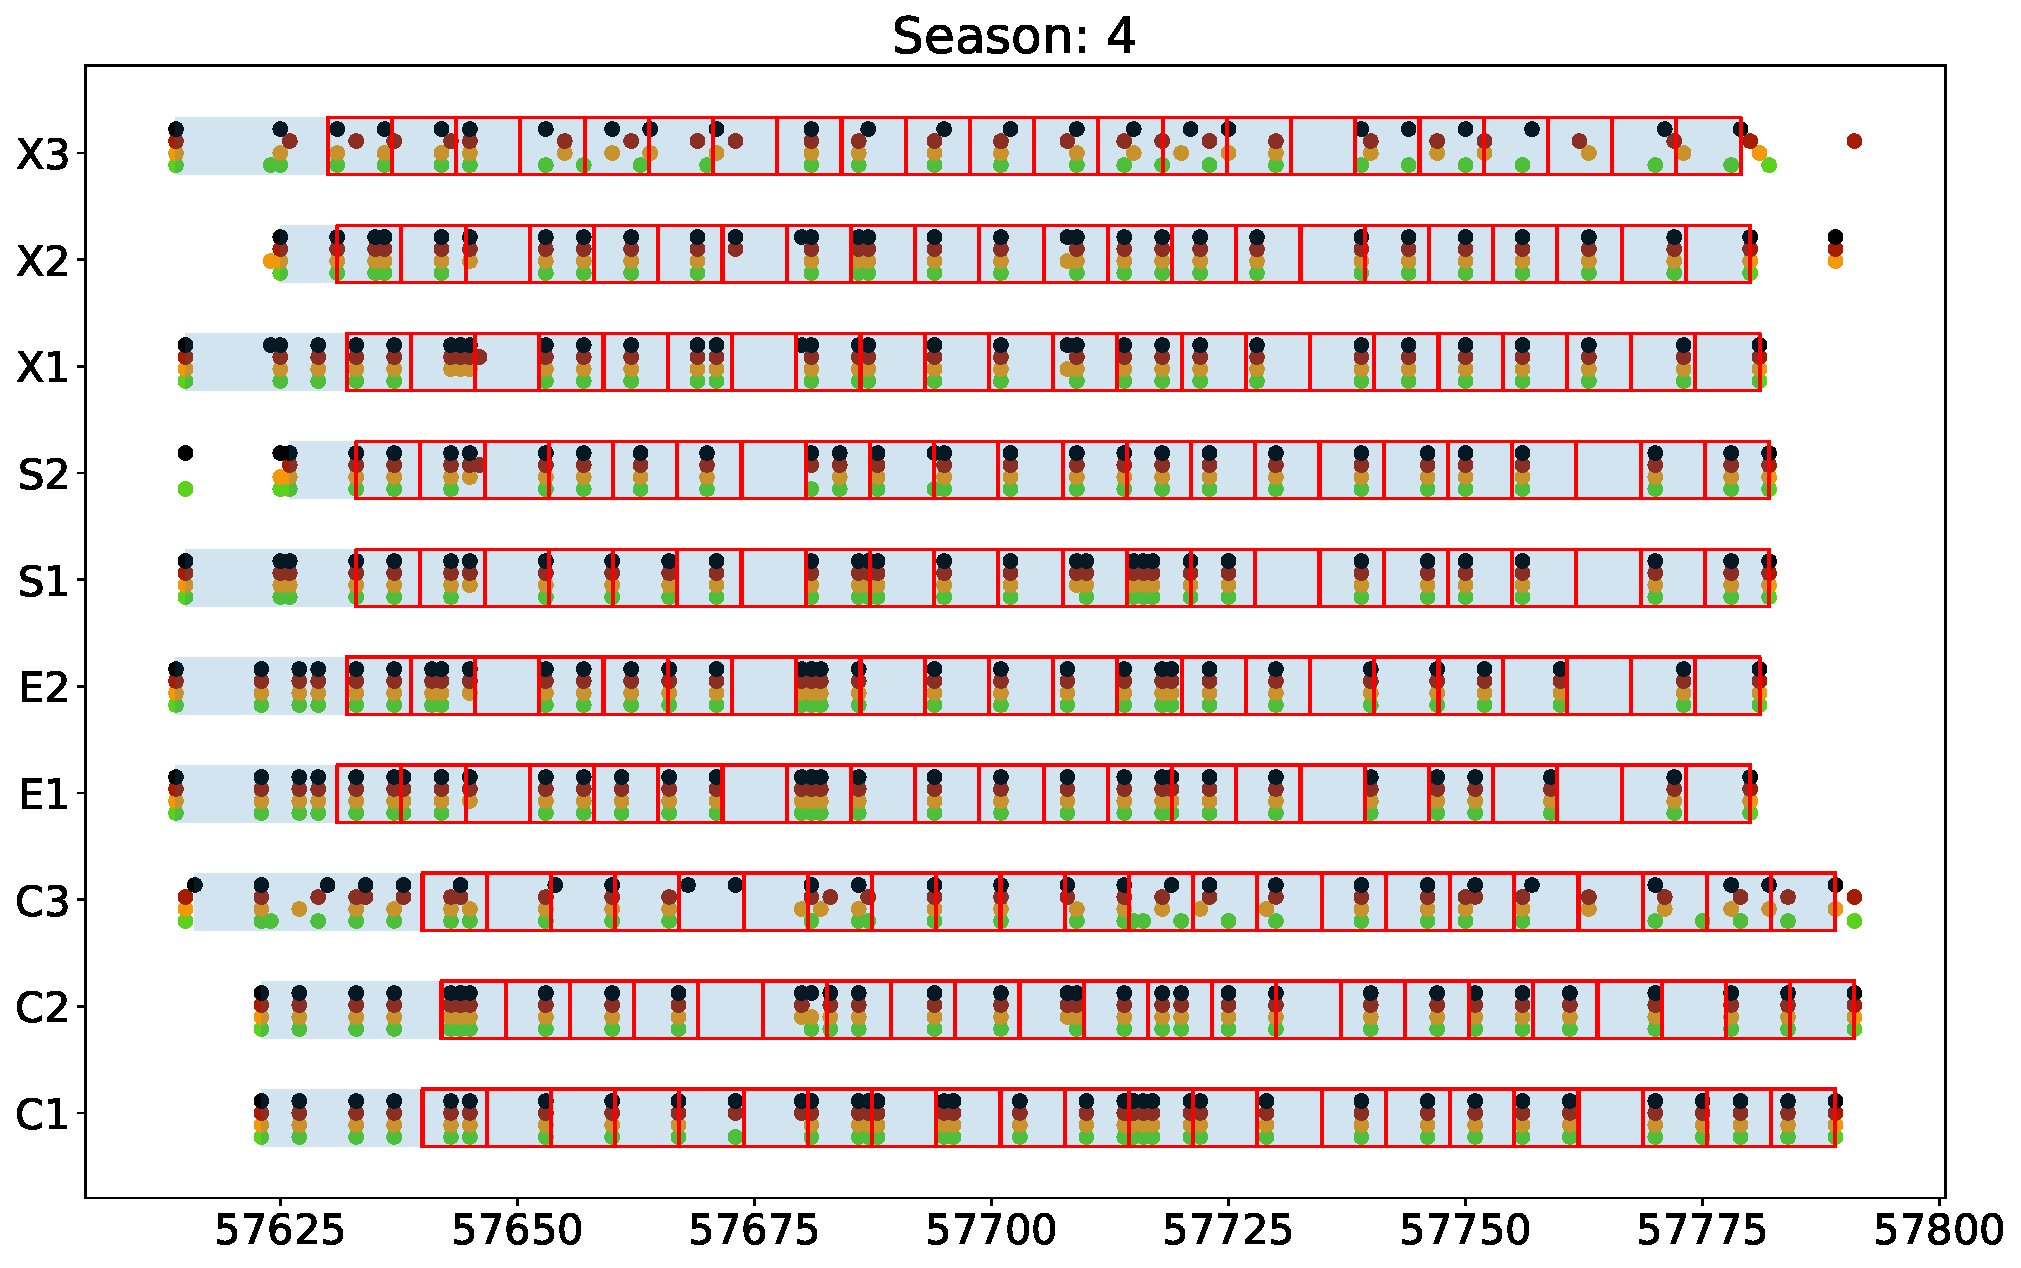
\includegraphics[width=\textwidth]{Figures/Chapter5/ObsBlock_Season4.pdf}
  \caption{}
  \label{fig:ObsBlock4}
\end{figure}

\subsection{Choosing the cadence} \label{sec:SimCadance}
Upon deciding on the observing block used in the simulations the next step I applied was was to decide on the cadance of the interpolated observations. As I am using GPRs I could apply essentially any cedence I want and there is no real rule for how much data should be included in the sample. I did however not want to either loose any information or use too many data points which would esentially only replicate the information that we already have.

The observed cadence of DES is not uniform and varies through the season due to the observing conditions. Early in the season, the cadence is shorter as the obseving weather conditions don't allow for the observatins of the wide DES fields leading to a shorter DES cadence as the deep and shallow fields are given more observing time. On the contrary, the cadence stabilised as the season progresses and settles at the designed 7 days. This is seen in \fref{fig:cadence} resulting in a bimodal distribution with an average cadance of 5 days. With a lack of any other factors that could help us decide on the cadence for the interpolated I use this value in \sref{sec:UseGP}.

\begin{figure}
  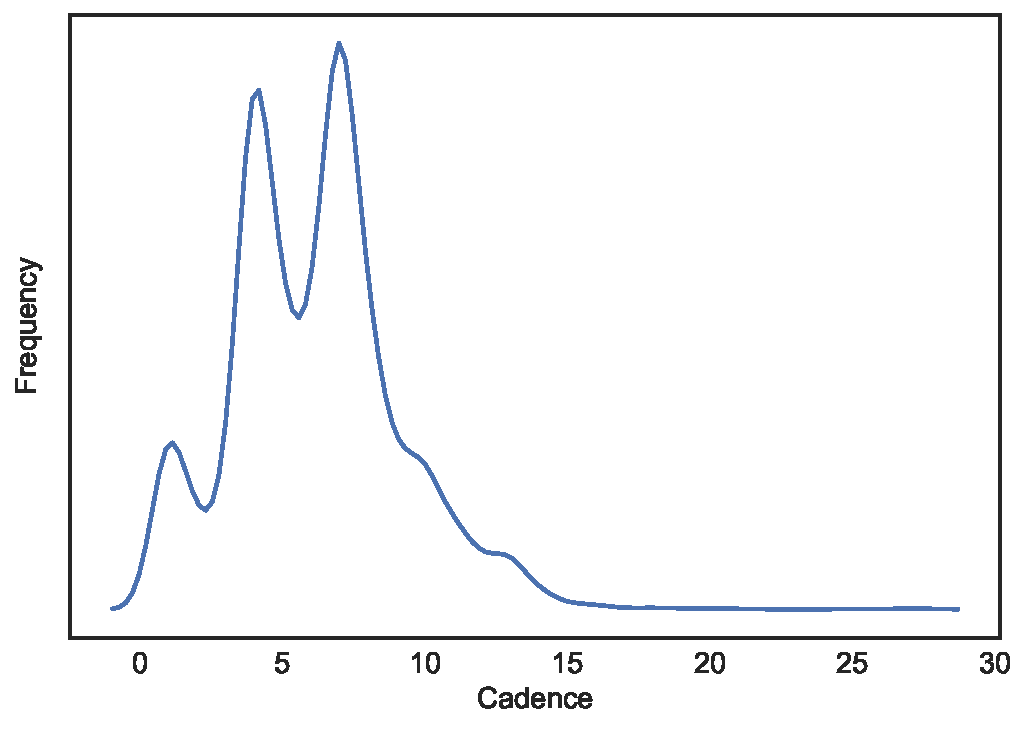
\includegraphics{Figures/Chapter5/Cadence.pdf}
  \caption{}
  \label{fig:cadence}
\end{figure}

\subsection{Applying Flux correction to Real Data}
Before the GPR can be applied to all the data it first needs to be corrected for the effects of DES switching the image subtraction template between season. As the focus of the DES SN team is predominantly the study of SN\,Ia they have always focused on maximising the quality of single season light curves. As the image quality has improved in the first two seasons of observations the templates have been updated each year. This is not an for the study of short transients where only a single season is of interest, however, for slowly evolving SNe (and AGNs) this causes an issue where the supernova light curve is present in the template result in decreased flux in the subsequent season. This is a particular problem for SLSN, where their evolution can often be slow enough to be detectable in multiple seasons in DES (Angus et al.; in prep). This may potentially be a strong factor in their classification and hence cannot be ignored.

While the most optimal approach to this would be to perform the image subraction and source detection with a single template this was both computationally prohibitive due to the scale and complexity of the raw DES data. As an alternative solution, I used the DES analysis logs to determine which observations have been used in the creation of the template images. In these frames, I measure the median flux of the object and use this value to correct the offset. As a simple test for this approach, I use a light curve of a SN\,Ia that explosed early in the second season of DES. In the uncorrected DES light curves this results in a flat but negative light curve in the third season. \fref{fig:FluxOffset} shows the original and corrected light curve, consistant with zero flux in the third season.

\begin{figure}
  % \includegraphics{/path/to/figure}
  \caption{}
  \label{fig:FluxOffset}
\end{figure}

\subsection{Applying GPs} \label{sec:UseGP}
The size and extend of the training sample used in this thesis is one of the two advancements made towards classifying SNe in DES using the ML approach. An equally important step, crucial for the use with CNNs, was the use of GPR (\sref{sec:GP}) as a tool for light curve interpolation and augmentation. CNN performs pattern recognision using a set of convolutional kernels with a fixed size, therefore requiring the data to be evenly sampled. This has tremendous benefits as it does not require any feature extraction steps and uses every data point in the classification process. While the observed data cannot be used directly in with this technique due to its non-uniform sampling, using a GP interpolated light curves removes less information about the data than a parametric model. Simulataniously, it does not introduces any correlations between the distinct bands, both in terms of the flux and the onset of the SN.

I apply the method described in \sref{sec:GP} to interpolate the light curves using the Mate\'rn 3/2 covarience functions. I perform the interpolation over the period selected in \sref{sec:ObsBlock} using the base cadence found in \sref{sec:SimCadance}. After testing the CNN in \sref{sec:CNN} I found that using a cadance which double the original 5 days, to 2.5 days, improves the accuracy of the model. The motivation behind the doubling of the cadance was to allow a gradiant for each point to be calculated closer to the point itself as opposed to between the points. The extra points act as control points in this scenario.

While the fitting correctly interpolated all of artifically generated light curves, it does fail for a small amound of real DES objects. I reviewed these visually and determined that this is caused by errors in the extraction where some points appear to have no uncertainty.

\section{Classifications} \label{sec:CNN}
The construction of the artificial DES training sample of transiants was a major step towards performing a comprehensive classification study using a machine learning approach. In recent years, the use of machine learning has expanded far beyond the purely academic uses within the field of Computer Science. The world around us is currently being shaped by AI augmented technologies driven in large measure by Artificial Neural Networks (ANN) and their derivatives such as Convoutional Neural Networks (CNN) and Deep Learning.

The process of selecting transients for spectroscopic follow-up is an example, albeit not explicit, of SN photometric classification. This task has been performed manually, through the visual inspection of the light curves, for decades in every SN survey. In recent years a number of attempts have been made to devise a pipeline for photometric classification of SN based on the clustering of light curve model parameters. However, this problem can be apprached from a more fundamental point of view using Artificial Intelligence (AI). Computer vision, a prominant branch of AI, has been successfully appliedd to countless examples of classification tasks where humans demonstrated a superiority over the early classification methods. Projects such as ImageNet [CITE] were able to produce models capable of identify a number of everyday entities (humans, vehicles, animals, household items) with an accuracy exceeding that of an average human. While the scarsity of the training samples available to us in comparison to projects such as ImageNet does not allow us to use an equally complex model, this is not requiered as the complexity and diversity of our transient data is not even a fraction as high as that of any everyday object.

In this section I describe the use of Convolutional Neural Networks (CNN) as an AI tool used to first identify SN light curves in the DES data and subsequently classify them into their respective subclasses with the overall aim of producing a photometric sample of DES SLSNe

\subsection{Convolutional Neural Networks}
CNNs are currently one of the most talked about topics in the world of AI and ML. While their wide spread use is novel and a result of the increase in the performance of computer devices, the theory behind them dates back to the early work on Artificial Neural Networks (ANN) [CITE, CITE] and replicating the ability of the human ability to learn based the external stimuli.

\subsubsection{Artificial Neural Networks}
All principle components of a ANN are fundamentally based on the human brain contain neurons, represented by nodes and activation functions. The nodes, usually aranged in a network of layers, are connected a set of weight which correstond to the biological synapsis. The aim of a ANN is to perform a non-linear transformation between the input parameters and the output values.

- Activation functions and weights
- Input output and hidden layers
- backpropagation and training

\subsubsection{Convolutional Neural Networks}
text

\subsection{SNe vs AGN vs Noise}
While CNNs are extremely powerful in their ability to classify images, regardless of what they contain, they often relie on huge amonuts of training samples in order to learn their discriminating qualities. In the case of DES transient data we are still not operating on a suffciently large dataset despite the work on enhancing the sample. However, it is possible to simplify the classification problem to reduce the amount of training samples required to produce a good classification score.

\subsubsection{Choosing the training sample} \label{sec:AGNNoiseSN}
As the first step in the analysis of the DES sample, I separate the task of classifying SN from that of identifying real SN transients amonst the background of spurious detections and AGNs also detected by the survey. As the traning sample for each class must be of similar shapes, I use all of the $\sim60000$ fake AGN generated in \sref{sec:AGN} as well as a random sample of 60,000 spurious noise examples. The matching SN sample must contain examples of all SN in approximatelly equal proportions. I therefore use 20,000 SN\,Ia, 10,000 SN\,Ibc, 10,000 SN\,II and 20,000 SLSN all drawn randomly from their simulated samples (\sref{sec:Augmentation}).

\subsubsection{Reshaping the data}
Due to their complexity, CNNs rely on heavily fine-tuned optimisers for minimising the model's loss functions. As a result, the data must satisfy a number of strict criteria in order to comply with these constrains. While most of them, such the need for the data to be linear, are naturally satisfied by the training dataset, we must observe a number of them including the upper and lower limits on the flux which must be in the range of positive and negative unity.

As the final piece of book-keeping, the data for all training samples must be concatinated into a single, multi-dimential matrix, shaped such as to separate the features which are dimentially independant of each order. In order to allow for the models described in the following section to extract both the colour and morphological evolution of the transients, each season of data is represented by a 4$\times$46, two dimentional vector, corresponding to the number of photometric bands and epoch per band respectively. This central block of data is build for each season independantly, as the large gap between the observing blocks means that the data cannot be treated as continuus.

\subsubsection{Designing the network} \label{sec:AGNNoiseModel}
The design of a neural network is often described as a dark art with no clear directions and and formalisims available as a guidline for the process. While some early work is taking place at Google in the area of optimising the morphology of the networks for maximum performance, this is a very computationally expensive task and therefore prohibitive for us. In the case of this thesis, I am instead relying on my domain knowladge of the distinquichable features of transients to perform the learning.

This has undergone many iterations with a wide range of layer complexity. In all instances, the first point of access in the model is a convolutional layer containing 30-80 independant filters each between 3-9 epochs wide. These filters are applied to each season and band independantly. A pooling layer is applied to the data at this point as a way of emphesising the features highlighted by the convolutional filters before a second convolutional layer, othogonal to the first layer, is applied to the data in order to measure the use the colour information at each epoch. At this stage, an average pooling layer is used again extracting the two most prominant features in the colour space for each filter.

After comparing a large number of iterations of these hyperparameters, I found that using 50 filters spanning 5 epochs in the first layer and 30 filters in the second layer were able to produce the highest accuracy. Perhapse counterintuitevely, iterations in which I combined these filters together did not provide a higher accuracy. A low number of orthogonal filters provide a freedom for the features to be learned independantly, and prevent the filters from relearning the same features. One could imagine a situation where a simiar light curve shape may be associated with a different colout evolution for different class of transients. This highlights the importance of allowing the CNN to build its own features out of the simplest building blocks without overcomplicating the design by constraining the model.

- Put in the schematics of the models

\subsubsection{Training the model}
The combined training sample build in \sref{sec:AGNNoiseSN} is passed through the network using a batch size of 5000 objects with 100 epoch, or individual runs of the backpropagation algorithm. CNNs are often trained on smaller batches of data to accelerate the learning process and help to prevent overfitting. The choice of the number of fitting epoch serves a similar, as a general rule of thumb the fitting is stopped when the model approaches convergence as an excesive number of epochs would allow the model to `learn' the test sample leading to overfitting.

My best model, as described in \sref{sec:AGNNoiseModel}, converges rapidly to the accuracy of 99.7\% which vastly exceeded our expectations. \fref{fig:AGNNoiseROC} shows the Receiver Operating Characteristic (ROC) which is the most commonly used metric of the accuracy of the classification model. [DESCRIBE WHAT ROC IS]. The ROC curve, in the case of this classifier, indocates that for each individual objects the probability of it being a true positive vs a true negative is 99.97\%.

\begin{figure}
  % \includegraphics{/path/to/figure}
  \caption{}
  \label{fig:AGNNoiseROC}
\end{figure}

\subsubsection{Selecting SNe}
After the numerous preparation steps we can now obtaining classifications for each real, unlabelled DES transient. 19,500 objects were sanitised and reshaped using the same method as the training sample before being passed thorugh the classification network. 6000 objects obtained the classification of `most-likely' being SN, e.g their probability of 

- I compare this to the sample of SNIa, CCSN, AGN and SLSNe and I find that all spectroscopically confirmed SN, regardless of their subclass are part of the sample while all objects which have been classifies as AGN have been identified as AGN. This is a trmendous result that trully shows that CNN are the perfect tool for this task and paves way to similar projects being used in future surveys including LSST.
- I decided to use a stricter cut at 99\% just to be sure which retained 5300 objects because all spec confirmed objects were at 99.5\% and over.

\subsection{Classifying SNe}
text
\subsection{SLSNe in DES}
